\documentclass[a4paper,12pt]{article}
\usepackage[utf8]{inputenc}
\usepackage[T1]{fontenc}
\usepackage[ngerman]{babel}
\usepackage{geometry}
% Anpassung der Ränder und des Header-Platzes, um fancyhdr-Warnungen zu vermeiden
\geometry{a4paper, left=2.5cm, right=2.5cm, top=3cm, bottom=3cm, headheight=15pt}
\usepackage{fancyhdr}
\usepackage{hyperref}
\usepackage{url}
\usepackage{listings}
\usepackage[dvipsnames]{xcolor}
\usepackage{pdfpages}
\usepackage{graphicx}


\lstset{
   literate={ö}{{ö}}1
           {ä}{{ä}}1
           {ü}{{ü}}1
           {ß}{{\ss}}1
           {é}{{\'e}}1,
   inputencoding=ansinew,
   extendedchars=true,
   basicstyle=\scriptsize\ttfamily,
   numberstyle=\scriptsize,
   breaklines=true,
   tabsize=4,
   numbersep=5pt
}
\lstdefinestyle{textstyle}{
    language={},                 % Verhindert blau markierte Wörter im Text
    basicstyle=\small\sffamily,  % Serifenlose Schrift (Arial-Look)
    breaklines=true,             % Automatischer Zeilenumbruch
    xleftmargin=0pt,             % Absolut keine Einrückung von links
    xrightmargin=0pt,            % Nutzt die volle Breite rechts
    frame=none,                  % Kein Kasten drumherum
    numbers=none,                % Keine Zeilennummern
    keepspaces=true,             % Behält deine Leerzeichen/Formatierung bei
    columns=fullflexible,        % WICHTIG: Erlaubt "normale" Buchstabenabstände
    literate={ä}{{ä}}1 {ö}{{ö}}1 {ü}{{ü}}1 {ß}{{\ss}}1 % Fix für Umlaute
}

\lstdefinestyle{customcpp}{
   language=C++,
   frame=single,
   numbers=left,
   keywordstyle=\color{blue}\bfseries,
   stringstyle=\color{BrickRed}\ttfamily,
   commentstyle=\color{OliveGreen}\ttfamily,
   showspaces=false,
   showstringspaces=false,
   showtabs=false,
   xleftmargin=5px
}

% Setup für Kopf- und Fußzeilen gemäß Vorlage
\pagestyle{fancy}
\fancyhf{} % Löscht Standard-Kopf-/Fußzeilen
\lhead{J. Rieger, L. Kieweg}
\chead{Systemdokumentation}
\rhead{Seite \thepage}
\renewcommand{\headrulewidth}{0.4pt}
\renewcommand{\footrulewidth}{0pt}

\begin{document}

%****************** self defined commands ***************************
%include a .cpp source file
%usage: \cppfile{../path_to_your_file/filename}
\newcommand{\cppfile}[1]{
\begin{itemize}
\item[]\lstinputlisting[label={lst:\detokenize{#1}}, style=customcpp,
    caption=\texttt{\detokenize{#1.cpp}}]{#1.cpp}
\end{itemize}
}

%include a .h source file
%usage: \hfile{../path_to_your_file/filename}
\newcommand{\hfile}[1]{
\begin{itemize}
\item[]\lstinputlisting[label={lst:\detokenize{#1}}, style=customcpp,
    caption=\texttt{\detokenize{#1.h}}
]{#1.h}
\end{itemize}
}

%include a module (.cpp and .h)
%usage: \hfile{../path_to_your_file/filename}
\newcommand{\cppmodul}[1]{
\begin{itemize}
\item[]\lstinputlisting[caption=#1.h,label="lst:#1-header", style=customcpp]{#1.h}
\item[]\lstinputlisting[caption=#1.cpp,label="lst:#1-impl", style=customcpp]{#1.cpp}
\end{itemize}
}

%include a code snippet
%usage: \hfile{../path_to_your_file/filename}{startline}{endline}
\newcommand{\snippet}[3]{
\begin{itemize}
\item[]\lstinputlisting[caption=#1.cpp,label="lst:#1-snip", style=customcpp, firstline=#2,lastline=#3]{#1.cpp}
\end{itemize}
}

%include a test-output file 
%usage: \testoutput{../path_to_your_file/filename}
\newcommand{\testoutput}[1]{
\begin{itemize}
\item[]\lstinputlisting[caption=#1]{#1.txt}
\end{itemize}
}

%include a figure -> ensure that the picture is in the pics directory
%usage: \fig{name_of_picture}{width}{caption text}
%width between 0.0 - 1.0 -> correspond with textwidth
\newcommand{\fig}[3]{
\begin{figure}[H]
\centering
\includegraphics[width=#2\textwidth]{pics/#1.PNG}
\caption{#3}
\label{fig:#1}
\end{figure}
}

\lstset{
   literate={ö}{{\"o}}1
           {ä}{{\"a}}1
           {ü}{{\"u}}1
           {ß}{{\ss}}1
           {é}{{\'e}}1,
   inputencoding=ansinew,
   extendedchars=true,
   basicstyle=\scriptsize\ttfamily,
   numberstyle=\scriptsize,
   breaklines=true,
   tabsize=4,
   numbersep=5pt
}

\lstdefinestyle{customcpp}{
   language=C++,
   frame=single,
   %backgroundcolor=\color{mygray},
   numbers=left,
   keywordstyle=\color{blue}\bfseries,
   stringstyle=\color{BrickRed}\ttfamily,
   commentstyle=\color{OliveGreen}\ttfamily,
   showspaces=false,
   showstringspaces=false,
   showtabs=false,
   xleftmargin=5px
}

% Angabe
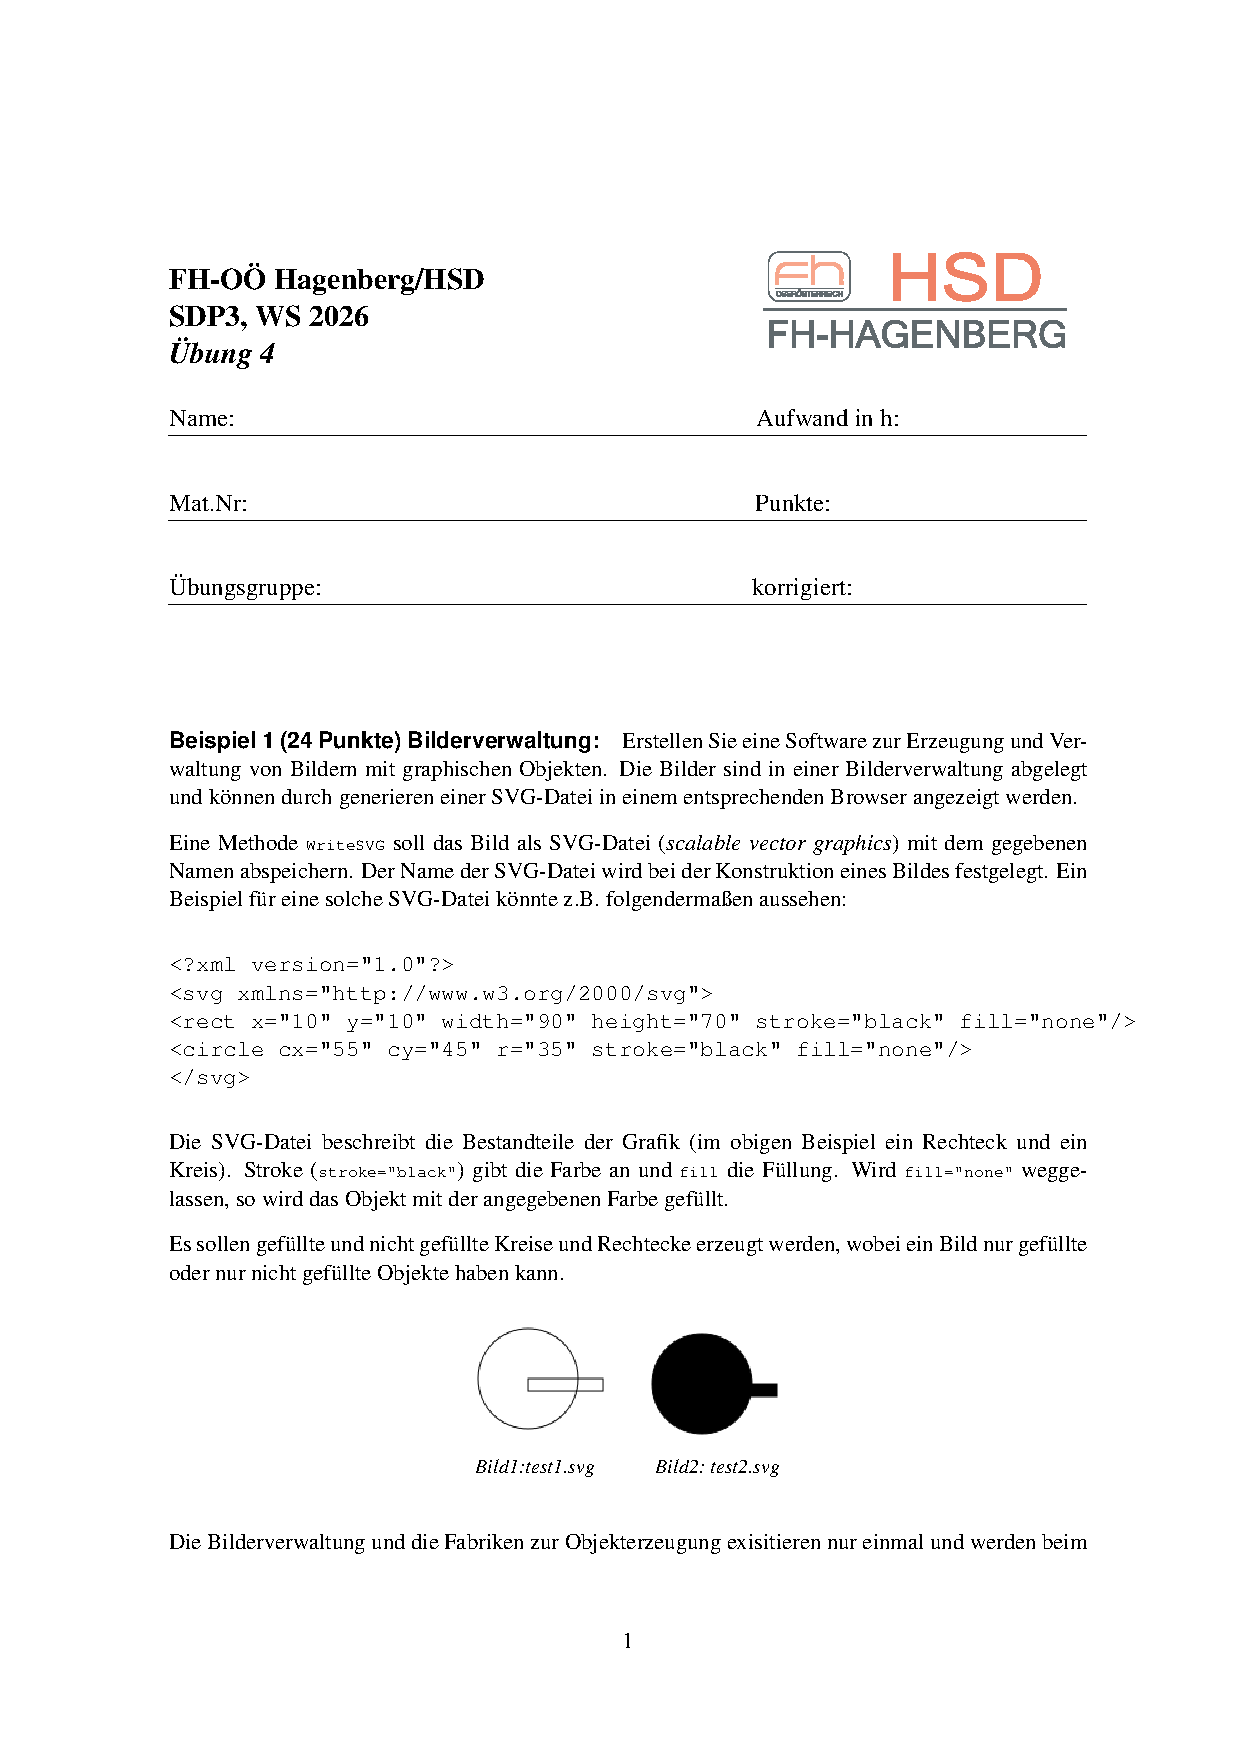
\includepdf[pages=-]{Angabe.pdf}



% -- Titelseite --
\begin{titlepage}
\vspace*{-1cm}
\noindent
HSD\\
OBERÖSTERREICH\\
FH-HAGENBERG

\vspace{4cm}
\begin{center}
{\Huge \textbf{Systemdokumentation}}\\[1cm]
{\Large \textbf{Player-Schnittstelle}}\\[0.5cm]
{\large Version 1.0}\\[2cm]
{\large J. Rieger, L. Kieweg}\\[0.5cm]
{\large Hagenberg, 28. Oktober 2026}
\end{center}

\vspace{3cm}
\noindent
Dieses Dokument zeigt den prinzipiellen Aufbau einer Systemdokumentation für Software-Projekte. Die einzelnen Kapitel sind mit Kommentaren versehen, welche die Struktur und den Inhalt erläutern.
\end{titlepage}

% -- Inhaltsverzeichnis --
\newpage
\tableofcontents
\newpage

% -- Kapitel 1 --
\section{Organisatorisches}
\subsection {Team}
\begin{itemize}
\item Julian Rieger, Matr.-Nr: S2510306023, E-Mail: S2510306023@fhooe.at
\item Leander Kieweg, Matr.-Nr: S2510306014, E-Mail: S2510306014@fhooe.at
\end{itemize}

\subsection{Aufteilung der Verantwortungsbereiche}
\begin{itemize}
\item Julian Rieger
    \begin{itemize}
        \item Implementierung der Klassen: Image, Object, GraphicObject, Circle, Rectangle, FillCircle, BlankCircle, FillRectangle, BlankRectangle
        \item Erstellen des Klassendiagramms
        \item Verfassen der Systemdokumentation
    \end{itemize}
\item Leander Kieweg
    \begin{itemize}
        \item Implementierung der Klassen: GraphicObjectFactory, FillGraphicObjectFactory, BlankGraphicObjectFactory, GraphicManagement
        \item Implementierung des Testtreibers

    \end{itemize}
\end{itemize}

\subsection{Aufwand}
\begin{itemize}
\item Julian Rieger: geschätzt: 10h, tatsächlich 9h
\item Leander Kieweg: geschätzt 10h, tatsächlich 9h
\end{itemize}

\newpage
% -- Kapitel 2 --
\section{Anforderungsdefinition (Systemspezifikation)}
Es wird eine Software zur Erzeugung und Verwaltung von Bildern mit grafischen Objekten erstellt. Ein Bild besteht aus gefüllten oder nicht gefüllten Kreisen und Rechtecken und kann als SVG-Datei gespeichert und in einem Browser angezeigt werden. Ein Bild enthält entweder nur gefüllte oder nur nicht gefüllte Objekte. Der Name der SVG-Datei wird bei der Konstruktion des Bildes festgelegt.
\subsection*{Funktionale Anforderungen}
\begin{itemize}
  \item \texttt{AddImage(fact, file)}: Legt ein neues Bild mit dem
        angegebenen Dateinamen an. Die übergebene Fabrik wird zur aktuellen
        Fabrik der Bilderverwaltung und erzeugt die Objekte dieses Bildes.
  \item \texttt{CreateCircle(stroke, x, y, radius)}: Erzeugt mit der aktuellen
        Fabrik einen Kreis (Mittelpunkt $(x,y)$) und fügt ihn dem zuletzt
        angelegten Bild hinzu.
  \item \texttt{CreateRectangle(stroke, x, y, width, height)}: Erzeugt mit der
        aktuellen Fabrik ein Rechteck (linke obere Ecke $(x,y)$) und fügt es
        dem zuletzt angelegten Bild hinzu.
  \item \texttt{WriteSVG()}: Schreibt alle Bilder der Bilderverwaltung als
        SVG-Datei. Ein einzelnes Bild kann ebenfalls über
        \texttt{Image::WriteSVG()} gespeichert werden.
  \item \texttt{ToSVG()}: Jedes grafische Objekt liefert sein SVG-Element als
        Text. Nicht gefüllte Objekte erhalten das Attribut
        \texttt{fill="none"}, bei gefüllten Objekten wird es weggelassen, sodass
        das Objekt mit der Strichfarbe gefüllt wird.
\end{itemize}

\subsection{Nichtfunktionale Anforderungen}
\begin{itemize}
  \item Bilderverwaltung und Fabriken existieren nur einmal (Singleton) und
        werden beim Programmende automatisch freigegeben.
  \item Grafische Objekte werden ausschließlich über eine Fabrik erzeugt.
        Kopieren und Zuweisen von Objekten ist verboten.
  \item Die Fabriken der Bilderverwaltung sind austauschbar, sodass
        verschiedene Bilder mit verschiedenen Fabriken erzeugt werden können.
  \item Das Design ist erweiterbar: Weitere Objektfamilien (z.B.
        schraffierte oder gepunktete Objekte) können ergänzt werden, ohne
        bestehende Klassen zu verändern.
  \item Für die SVG-Datei muss keine Grammatik angegeben werden.
\end{itemize}


\subsection*{Fehlerbehandlung}
Fehler werden als Ausnahmen (\texttt{std::exception}) gemeldet und vom
Testtreiber abgefangen und per \texttt{std::cerr} ausgegeben:
\begin{itemize}
  \item \texttt{std::logic\_error}, wenn \texttt{CreateCircle} oder
        \texttt{CreateRectangle} aufgerufen wird, ohne dass eine Fabrik gesetzt
        oder ein Bild angelegt wurde.
  \item \texttt{std::runtime\_error}, wenn eine SVG-Datei nicht geöffnet
        werden kann.
\end{itemize}
\newpage
% -- Kapitel 3 -- 
\section{Systementwurf}
\subsection{Klassendiagramm}

\begin{figure}[htbp]
  \centering
  \makebox[\textwidth][c]{%
    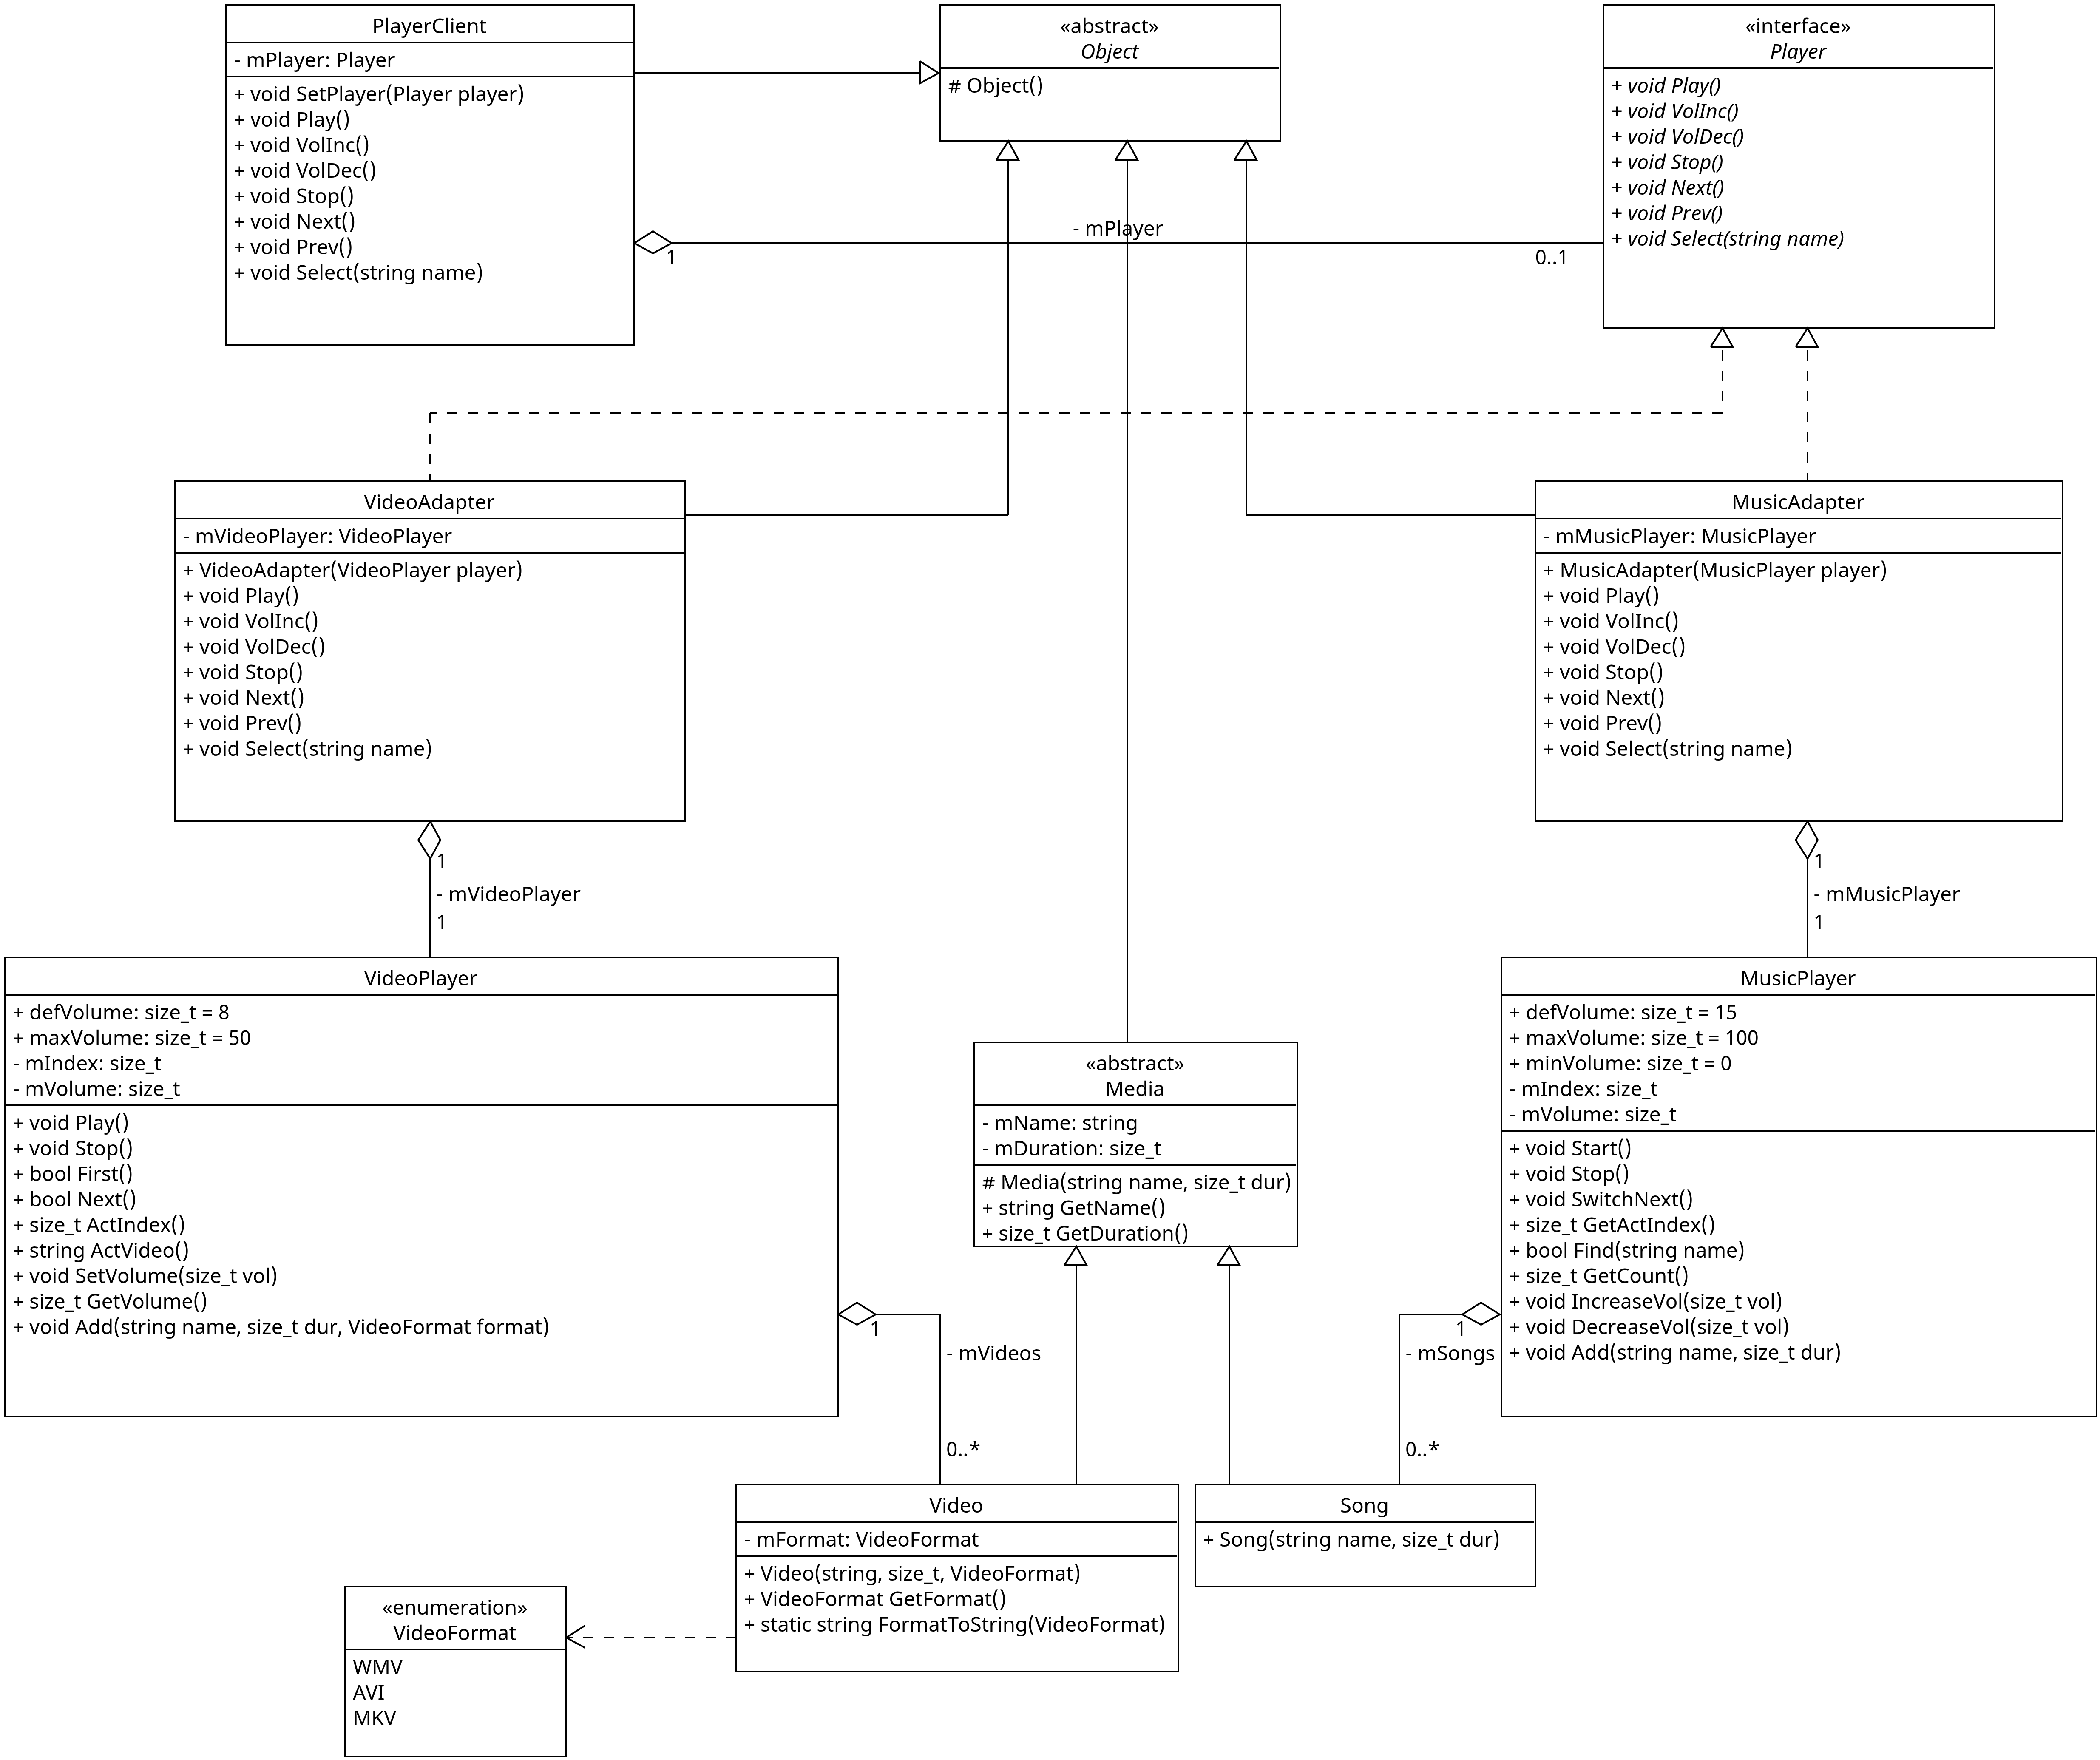
\includegraphics[width=1.0\textwidth]{diagramm}%
  }%
  \caption{Klassendiagramm Bilderverwaltung}
  \label{fig:klassendiagramm}
\end{figure}
Anmerkung: Das Klassendiagram steht für bessere Lesbarkeit ebenfalls im Sysdoku-Ordner zur Verfügung.

\newpage
\subsection{Designentscheidungen}
Für die Bilderverwaltung wurden folgende Entwurfsmuster eingesetzt, um Erweiterbarkeit und lose Kopplung zu gewährleisten.

\paragraph{Abstract-Factory-Pattern}
Die Schnittstelle \texttt{IGraphicObjectFactory} beschreibt die Erzeugung einer Familie zusammengehöriger Objekte (Kreis und Rechteck). Die konkreten Fabriken \texttt{BlankGraphicObjectFactory} und \texttt{FillGraphicObjectFactory} erzeugen jeweils nur nicht gefüllte bzw. nur gefüllte Objekte. Dadurch kann ein Bild nie beide Arten mischen. Die \texttt{GraphicManagement} kennt nur die Schnittstelle und die abstrakten Produkte \texttt{Circle} und \texttt{Rectangle}. Neue Familien (z.\,B. \texttt{HatchedGraphicObjectFactory} mit \texttt{HatchedCircle} und \texttt{HatchedRectangle}) können ergänzt werden, ohne bestehenden Code zu ändern. Die Fabrik ist pro Bild austauschbar (Parameter von \texttt{AddImage}).

\paragraph{Singleton-Pattern}
Bilderverwaltung und konkrete Fabriken dürfen nur einmal existieren. Dazu dient die Template-Klasse \texttt{SingletonBase<T>}: Die Instanz wird beim ersten Aufruf von \texttt{GetInstance()} erzeugt und in einem statischen \texttt{std::unique\_ptr} gehalten. Sie wird dadurch beim Programmende automatisch freigegeben (\texttt{Delete()} erlaubt zusätzlich eine vorzeitige Freigabe). Die Konstruktoren der Singletons sind privat bzw. geschützt, die Basisklasse ist dazu als \texttt{friend} eingetragen.

\paragraph{Vererbungshierarchie und Kopierverbot}
Alle Klassen leiten direkt oder indirekt von \texttt{Object} ab. Dessen Kopierkonstruktor und Zuweisungsoperator sind gelöscht, womit das Kopieren und Zuweisen aller abgeleiteten Klassen verhindert wird. Der geschützte Konstruktor verhindert die direkte Instanziierung.

\paragraph{Gemeinsame Basisklassen der grafischen Objekte}
Gemeinsame Attribute (Strichfarbe, Position) liegen in \texttt{GraphicObject}, die geometrischen Eigenschaften in \texttt{Circle} bzw. \texttt{Rectangle}. Die Unterklassen unterscheiden sich nur in \texttt{ToSVG()} (Polymorphismus). Die Konstruktoren der Basisklassen sind geschützt, die Objekte werden nur über die Fabriken erzeugt.

\paragraph{Besitzverhältnisse}
Die Fabriken geben \texttt{std::unique\_ptr} zurück. Das \texttt{Image} besitzt seine Objekte, die \texttt{GraphicManagement} besitzt die Bilder und hält die aktuelle Fabrik nur als nicht besitzenden Zeiger (die Fabriken sind selbst Singletons).

\paragraph{Fehlerstrategie}
Ungültige Aufrufe (keine Fabrik oder kein Bild vorhanden, Datei nicht
beschreibbar) werden über Ausnahmen gemeldet und im Testtreiber behandelt.
% -- Kapitel 4 --
\section{Komponentenentwurf}
Die HTML-Startdatei befindet sich im Verzeichnis ./../doxy/html/index.html

\newpage
% -- Kapitel 5 --
\section{Testprotokollierung}
\subsection{Ausgabe Konsole Testtreiber}
\begin{lstlisting}[style=textstyle]
Created blank-cyberpunk.svg and filled-cyberpunk.svg
\end{lstlisting}

\subsection{Erstellte Bilder}
\begin{figure}[htbp]
  \centering
  \makebox[\textwidth][c]{%
    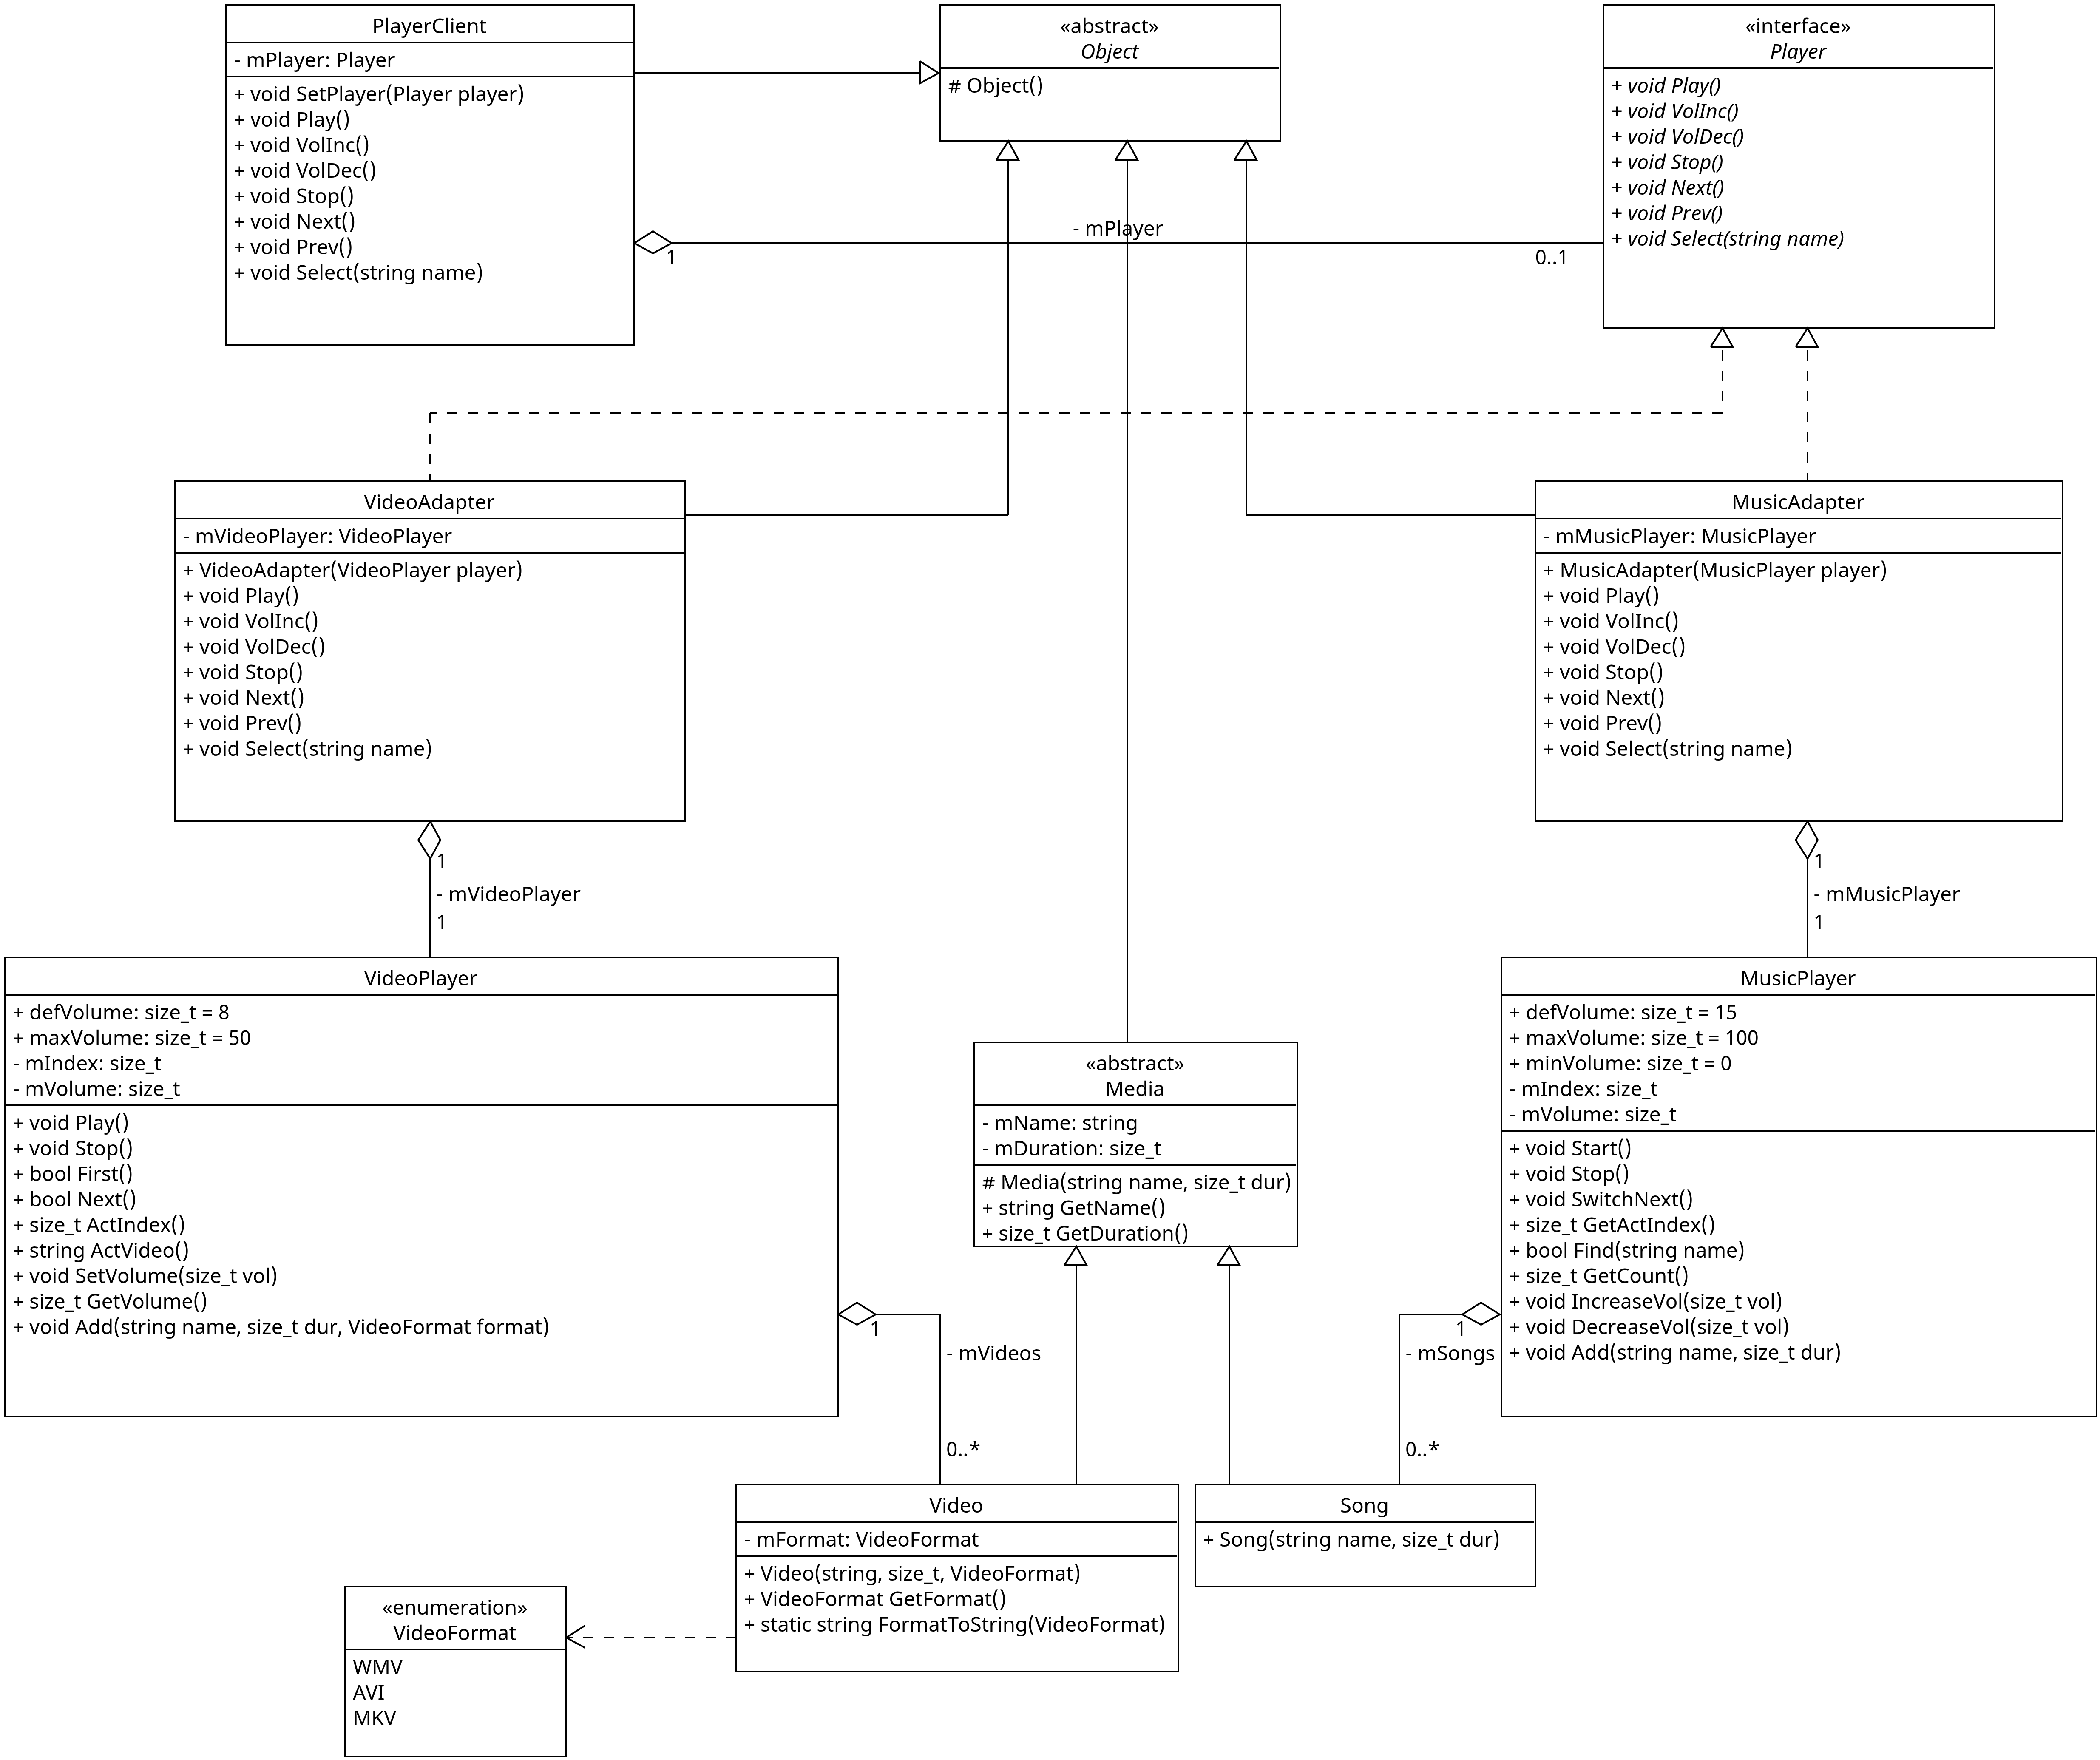
\includegraphics[width=1.0\textwidth]{diagramm}%
  }%
  \caption{Klassendiagramm Bilderverwaltung}
  \label{fig:klassendiagramm}
\end{figure}
\begin{figure}[htbp]
  \centering
  \makebox[\textwidth][c]{%
    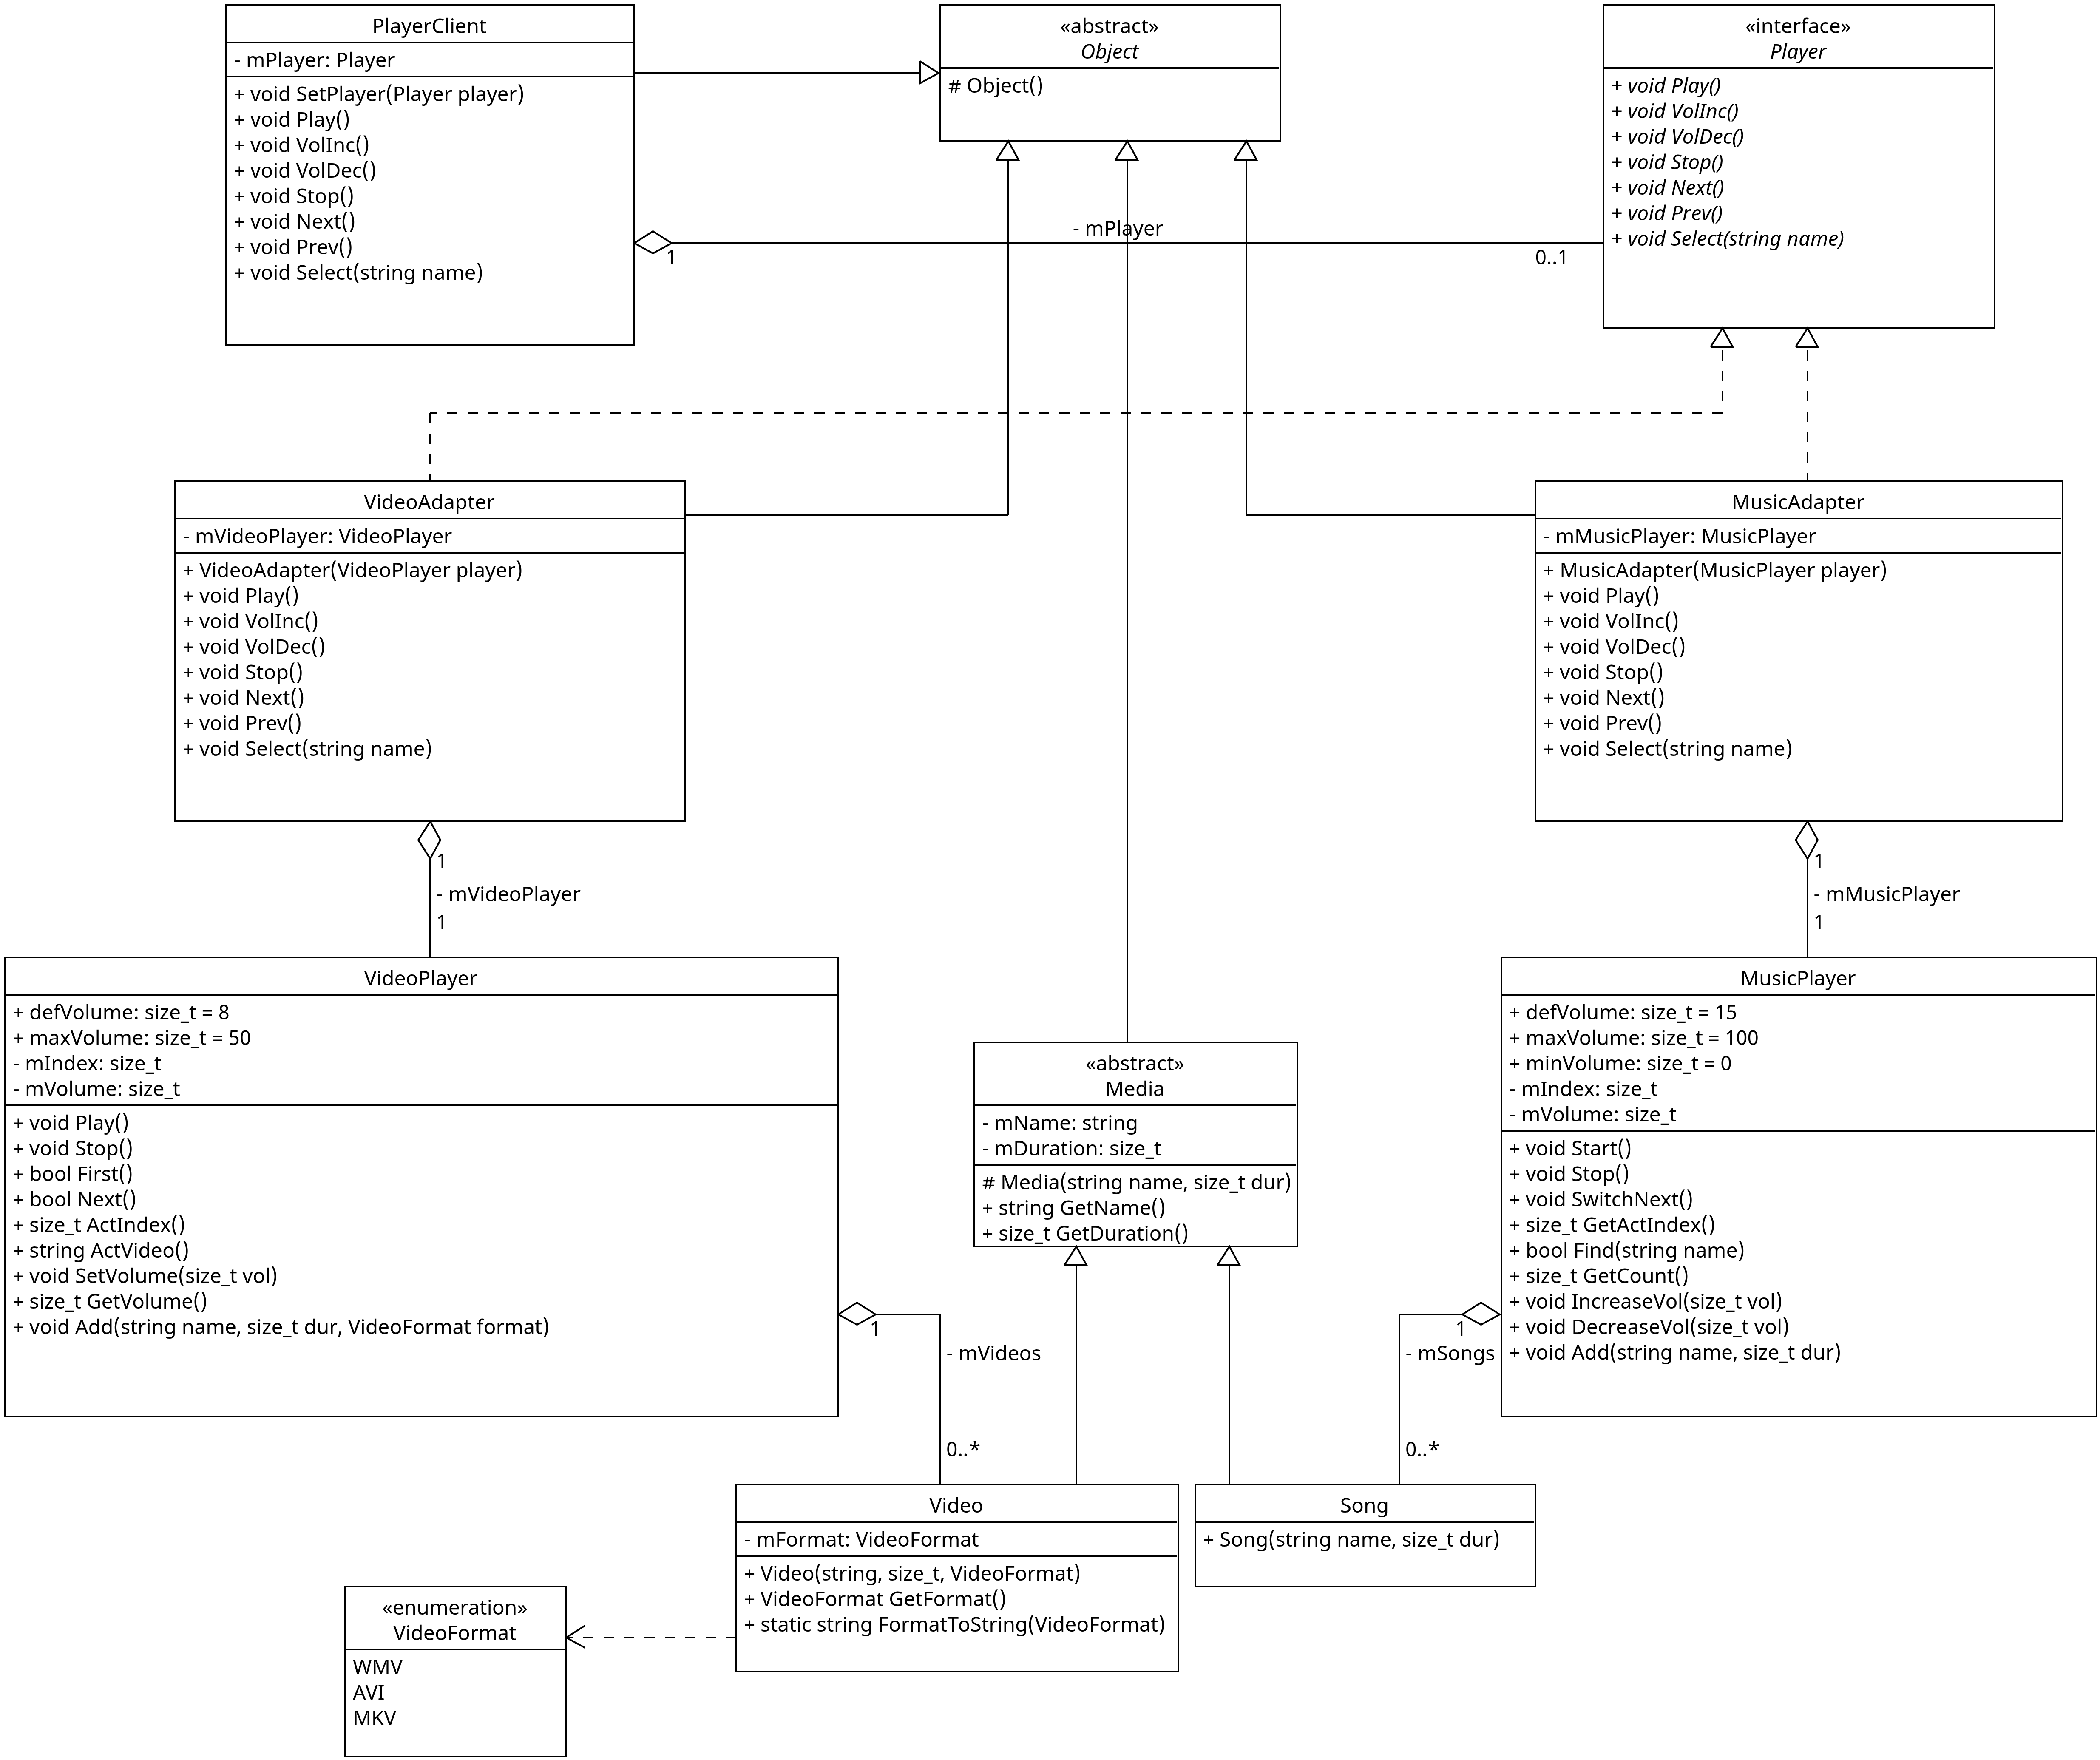
\includegraphics[width=1.0\textwidth]{diagramm}%
  }%
  \caption{Klassendiagramm Bilderverwaltung}
  \label{fig:klassendiagramm}
\end{figure}

% -- Kapitel 6 --
\newpage
\section{Quellcode}
\hfile{../Object}
\hfile{../BlankCircle}
\cppfile{../BlankCircle}
\hfile{../FillCircle}
\cppfile{../FillCircle}
\hfile{../Circle}
\cppfile{../Circle}
\hfile{../BlankRectangle}
\cppfile{../BlankRectangle}
\hfile{../FillRectangle}
\cppfile{../FillRectangle}
\hfile{../Rectangle}
\cppfile{../Rectangle}
\hfile{../SingletonBase}
\hfile{../IGraphicObjectFactory}
\hfile{../BlankGraphicObjectFactory}
\cppfile{../BlankGraphicObjectFactory}
\hfile{../FillGraphicObjectFactory}
\cppfile{../FillGraphicObjectFactory}
\hfile{../Image}
\cppfile{../Image}
\hfile{../GraphicManagement}
\cppfile{../GraphicManagement}
\cppfile{../main}
\end{document}